\documentclass[11pt]{article}
\usepackage[utf8]{inputenc}
\usepackage{graphicx}
\usepackage{verbatim}
\usepackage{listings}
\usepackage{mathtools}
\lstset{language=C, frame=single}

\topmargin=-15mm
\oddsidemargin=0mm
\textwidth=159.2mm
\textheight=220mm

\title{Home Exam 2: Video Encoding on the Cell Broadband Engine}
\author{Paweł Kozłowski \and Łukasz Mazurek}


\begin{document}
\maketitle

\section{Introduction}
We have implemented some optimizations of \texttt{codec63} encoder.
We focused on using the parallelization potential in motion estimation and and \emph{dct} quantization,
because these two parts of the code are the slowest.

\section{Motion vector searching}
\begin{itemize}
\item
The first observation was that the program spends more than 90\% on its
duration time on searching for motion vector.
\item
Implemented algorithm (\emph{full search}) checks 1024 candidates for motion vector for each $8 \times 8$ block.
For every motion vector candidate it calculates the costly \emph{SAD} function
between the corresponding $8 \times 8$ block of original and reference image.
The vector with the lowest \emph{SAD} value is choosed as a motion vector.
In other words, the task is to find a minimum of $SAD(x,y)$ function
over an area of $x,y \in \{-16, \ldots, 15\}$.
\end{itemize}

\subsection{Diamond search algorithm}
We decided to change the \emph{full search} algorithm to \emph{diamond search}\cite{ds} algorithm.
This algorithm is based on observation that for most pictures the 
$SAD(x,y)$ function changes slowly and continuously from pixel to pixel.
Therefore, we can always search for minimum in a direction of the biggest
 decrease of \emph{SAD} function.

\begin{figure}[h]
    \centering
    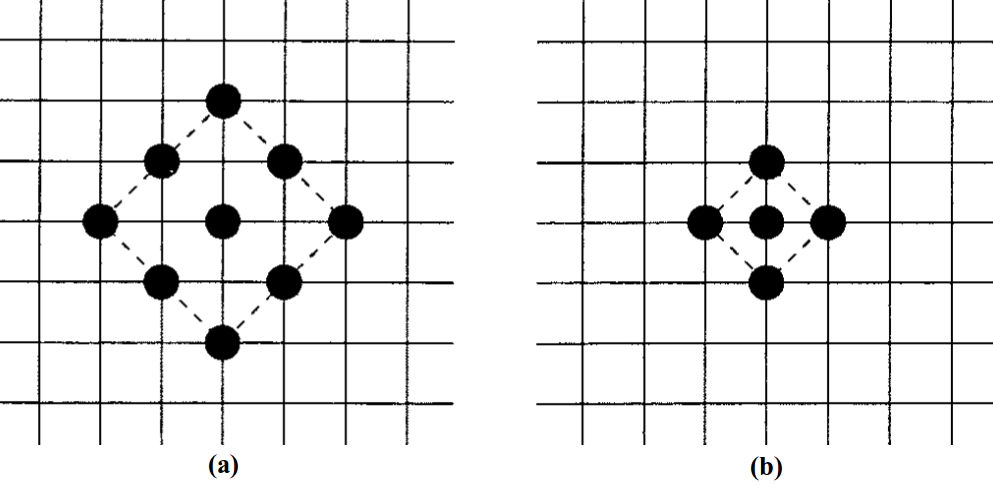
\includegraphics[width=0.6\textwidth]{bigsmall}
    \label{bigsmall}
    \caption{\textbf{(a)} Large diamond search pattern (LDSP), \textbf{(b)}
    Small diamond search pattern (SDSP)}
\end{figure}

More precisely, \emph{Diamond search} algorithm starts with coordinates of 
reference block equal to coordinates of original block.
In each step of algorithm we calculate
(or reuse the already calculated) the \emph{SAD} value in the current
position and the 8 neighbouring positions according to \emph{large diamond
search pattern} (\emph{LDSP}, fig. 1 (a)).
I next step we move our reference block in the direction of the lowest 
\emph{SAD} value and repeat the procedure.

Whenever the \emph{SAD} value in the current position is lower than
in all the neighbouring points, we approximately found a minimum.
Then we can calculate \emph{SAD} values in the 4 closer neighbors 
according to \emph{small diamond search pattern} (\emph{SDSP}, fig. 1. (b))
in order to find the exact position of the minimum.

Note that in each step the \emph{SAD} value is not increasing and therefore
algorithm is guaranteed to stop (we can easily avoid falling into a cycle
in case of equal \emph{SAD} valuse).
Although there is a possibility to stick in local minimum and not find the
global minimum,
the experiments\cite{ds} show that in case of typical movies this algorithm
usually leads to obtain the global minimum.

\subsection{Parallelization of motion vector search}
Even after a change of \emph{full search} to \emph{diamond search}
algorithm, the motion estimation is still the slowest part of encoder.
Therefore we decided to optimize this procedure in the following way:
\begin{itemize}
\item
Calculating the motion vector for each $8 \times 8$ block is independent. 
Therefore we can process 6 blocks at once, each on separate SPU.
\item
Calculating of \emph{SAD} of two $8 \times 8$ block can be easily rewrited into 
vector operations --- \emph{SAD} of 1-byte numbers with one \texttt{spu\_absd}
instruction.
\end{itemize}
After these optimizations the most time of each SPE was spent on wating for next
task from PPE.
That was because PPE was dealing tasks consequently:
\begin{itemize}
\item task nr 0 for SPE 0, 
\item task nr 1 for SPE 1,\\
 $\vdots$
\item task nr 5 for SPE 5,\\
$\vdots$
\item task nr 6 for SPE 0\\
$\vdots$
\end{itemize}
It can be inefficient way for distributing tasks, because each instance
of \emph{diamond search} algorithm can last in very different time.
Therefore, after a fast found of motion vector SPE must wait until the other
SPEs finish their job and get their next tasks.

We optimized this procedure in the following way: after finishing of previous job,
the SPE gets the next block to process itself.
Thus, SPE doesn't have to wait for other cores --- whenever there is a task to do,
it gets the task and doesn't waste its time for waiting.

Another observation was that the SPE spends most time on reading the $39 \times 39$
block of reference image, which is needed to search for a motion vector in the whole
range of 16 pixels in each direction.
However, in many cases motion vector is found closer than 16 pixel from the origin,
so we don't need the whole $39 \times 39$ data of reference image.
Therefore we can read this data row-by-row, only when a particular row is necessary
to compute the \emph{SAD} function.
This optimization also improved the speed of motion estimation significantly.

\section{DCT quantization}
DCT quantization is the second most costly part of the algorithm, so we decided
to parallelize it too.
Since DCT quantization can be done independantly for each $8 \times 8$ block,
we can distribute this calculation into SPEs similarly to motion estimation.
We can also easily rewrite all the calculation into the vector calculation,
which improves the program speed significantly.

\section{Bug in precode --- size of frame not divisible by 16}
We spent a lot of time on debugging the very strange segmentation fault during
encoding the \texttt{tractor.yuv} movie.
The problem was that the height of \texttt{tractor.yuv} movie is 1080, which is
not divisible by 16.
The precode seemed to deal with movies of any size, because \textbf{almost} every
array size was rounded up to the value divisible by 16.
Unfortunately the \texttt{in\_data} read from the input file wasn't.
Therefore the \emph{dct\_quantize} function was processing the rows 1080--1087
of output data using rows 1080--1087 of input data which where outside the allocated
memory.

\section{Summary}
We implemented some optimizations which improved the speed of \emph{c63} encoder.
On of the two most noticable changes were change the algorithm of motion vector finding from full search to diamond search.
Another noticable change was parallelization of \emph{motion estimation} and \emph{dct quantization} procedures.
Parallelization means in this case using 6 SPE cores to perform simultaneous computation and
using vector (instead of scalar) calculation.

\begin{thebibliography}{9}
\bibitem{ds}
Shan Zhu, Kai-Kuang Ma,
\emph{A New Diamond Search Algorithm for Fast Block-Matching Motion Estimation,}
IEEE transactions on image processing, vol. 9, No. 2,
February 2000

\end{thebibliography}

\end{document}
